\documentclass{report}

\usepackage[utf8]{inputenc}
\usepackage[T1]{fontenc}
\usepackage[francais]{babel}
\usepackage{listings}
\usepackage[a4paper]{geometry}
\usepackage{graphicx}
\usepackage[export]{adjustbox}
\usepackage{titlesec}
\usepackage{color}
\usepackage[toc, page]{appendix}
\usepackage{hyperref}

\definecolor{xcodekw}{rgb}{0.75, 0.22, 0.60}
\definecolor{xcodestr}{rgb}{0.89, 0.27, 0.30}
\definecolor{xcodecmt}{rgb}{0.31, 0.73, 0.35}

\titleformat{\chapter}[display]
  {\centering\normalfont\huge\bfseries}
  {\chaptertitlename\ \thechapter}
  {20pt}
  {\Huge}

\geometry{hscale=0.75,vscale=0.85,centering}

\DeclareUnicodeCharacter{00A0}{ }

\lstset{
  frame=tb,
  language=C,
  aboveskip=3mm,
  belowskip=3mm,
  showstringspaces=false,
  columns=flexible,
  basicstyle={\small\ttfamily},
  numbers=none,
  breaklines=true,
  breakatwhitespace=true,
  tabsize=3,
  keywordstyle=\color{xcodekw},
  stringstyle=\color{xcodestr},
  commentstyle=\color{xcodecmt}
}

\renewcommand{\thesection}{\arabic{section}}
\renewcommand\appendixtocname{Annexes}
\renewcommand\appendixname{Annexes}
\renewcommand\appendixpagename{Annexes}

\title{Projet OS}
\author{Youri \bsc{Mouton}, Rémy \bsc{Voet} et Samuel \bsc{Monroe}}
\date{Janvier 2015}

\begin{document}

\maketitle

\chapter{Introduction}

	\section{Introduction}

		Le projet qui fait l'objet de ce rapport est un travail de programmation
		en C système sous UNIX, dans le but d'exploiter de manière pratique les connaissances théoriques acquises au cours de Mme. Masson.
		\newline

		Ce travail consiste en l'écriture de trois programmes distincts autour d'une thématique aéronautique, échangeant des informations entre eux via divers moyens, ceci tout en gérant les éventuels conflits et erreurs liés à ces échanges.\newline
		Ces trois programmes sont :\newline
		\begin{description}
			\item[Tour de controle : ]
			Fait office de \textbf{serveur}, joue le rôle majeur en s'occupant de recevoir les demandes des pilotes, en allant chercher les informations météo fournies par le centre météo, et en renvoyant celles-ci en tant que réponses aux demandes des pilotes.\newline

			\item[Pilote : ]
			Fait office de \textbf{client}, envoie une demande d'information ATIS à la tour de contrôle, récupère cette information et replace une demande si cette information n'est pas intègre.\newline

			\item[Le centre météo : ]
			Programme \textbf{tiers} dans l'application, celui-ci se charge de générer automatiquement des informations ATIS différentes tout au long de son fonctionnement.\newline
		\end{description}

	\section{Rappel de l'énoncé}

		Des pilotes qui souhaitent décoller d’un aéroport non contrôlé ont besoin, pour ce faire, de connaître les informations ATIS. Celles-ci sont accessibles via un serveur.
		Chaque pilote va envoyer au serveur une demande ATIS. Le serveur va lors répondre à cette demande en allant chercher les informations nécessaires dans un fichier ATIS.
		Le pilote va recevoir ces informations et il doit alors obligatoirement répondre au serveur en lui envoyant soit :\newline
		\begin{itemize}
			\item Un ACK OK qui signifie \og informations bien reçues \fg et provoque la fin de la communication
			\item Un NAK KO qui signifie \og informations mal comprises \fg et nécessite de renvoyer les informations.
		\end{itemize}

		Le serveur doit pouvoir gérer un nombre indéfini de pilotes (restons réalistes).
		Le fichier ATIS contenant les informations nécessaires aux pilotes doit être régulièrement mis à jour par le gestionnaire météo.

\chapter{Analyse}

	\section{Plan global de l'application}
		Voici un schéma donnant un aperçu rapide des fichiers constituant l'application, et les interactions entre eux via des liens légendés : \newline

		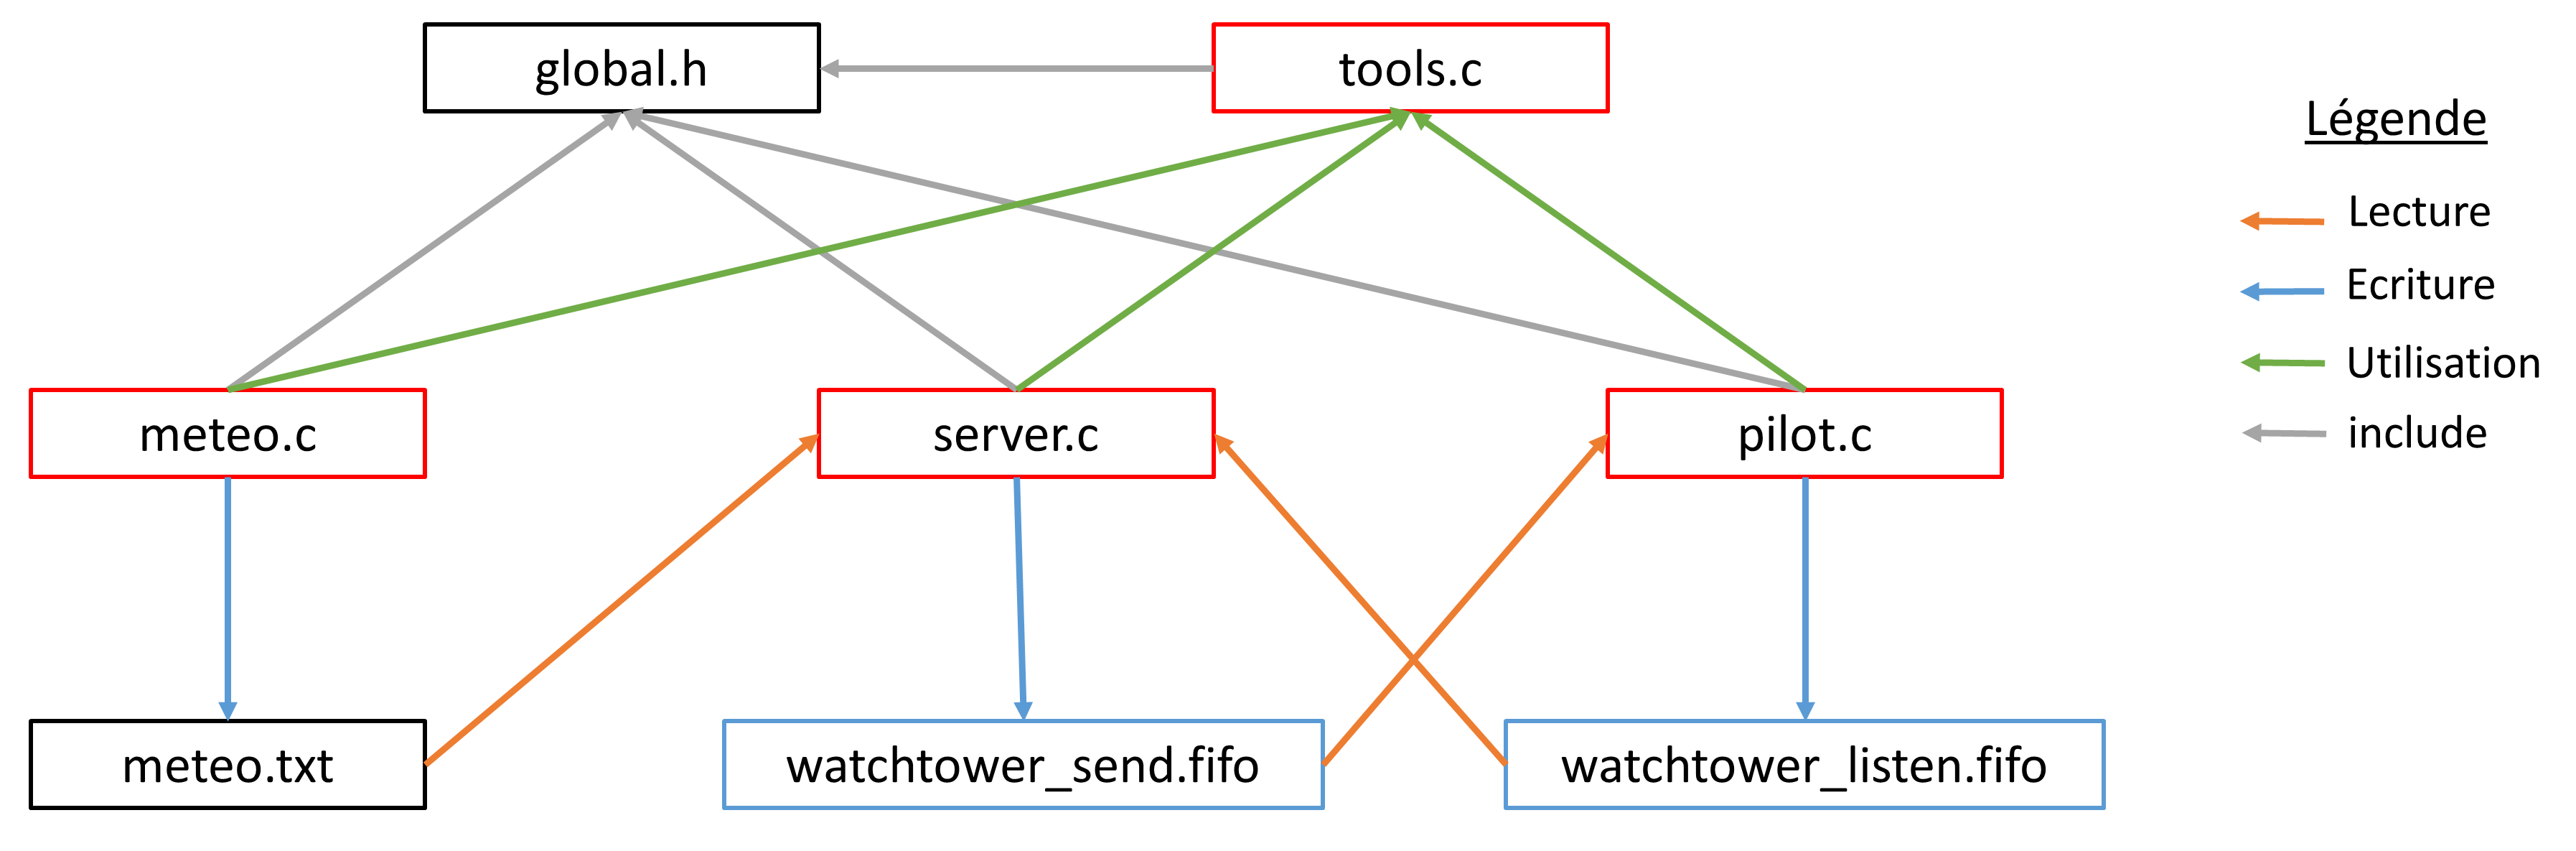
\includegraphics[width=\linewidth, frame]{schemasProjet.png} \newline

		Nos trois programmes qui constituent le coeur de l'application se trouvent sur la ligne au {\textbf{milieu} du schéma, écrits dans les fichiers {\textbf{\color{red} server.c}}, {      \textbf{\color{red} pilot.c}} et {\textbf{\color{red} meteo.c}}.

		Ces programmes vont se servir d' \og outils \fg fonctionnalisés dans le fichier {\textbf{\color{red} tools.c}} et obtenir les librairies, déclarations des fonctions outils et constantes  via inclusion du fichier {\textbf{\color{black} global.h}}.

	\section{meteo.c}

		Lors de la mise en route de l'application, nous commençons par lancer le contrôleur météo.
		Celui-ci possède en son sein un certain nombre d'informations ATIS différentes à utiliser.
		Le contrôleur météo fonctionne sur une succession de boucles, dans lesquelles il va :

		- Sélectionner aléatoirement une des informations ATIS qu'il possède en mémoire.

		- Créer un fichier de verrouillage nommé "lock", afin de spécifier à son environnement qu'il est en train d'opérer.

		- Le contrôleur ouvre ensuite le fichier "meteo.txt" qui va contenir l'information ATIS actuelle destinée aux autres programmes, si ce fichier n'existait pas, Meteo le crée.

		- Si l'ouverture est un succès, météo écrit l'ATIS généré précédemment sur le fichier, ceci en troncature de manière à éliminer une autre information ATIS qui est le résultat d'une opération précédente. Cette écriture va durer une seconde, seconde définie par nos soins.

		- Si l'écriture s'est bien déroulée, météo supprime le fichier de verrouillage "lock" pour spécifier à l'environnement que l'écriture est terminée et que "meteo.txt" est accessible, et termine la boucle après un repos défini de deux secondes.
\clearpage
\textbf{Pseudo-code}

\begin{lstlisting}[language=C]
Tantque NonArret
		Texte ATIS = ChoixATISAleatoire
		CreationFichierVerrouillage
		OuvrirFicherMeteo
		EcrireMeteoATIS
		FermerFichierMeteo
		DestructionFichierVerrouillage
		AttendreUneSeconde
Fin tantque 
\end{lstlisting}

	\section{server.c}

		Après l'ouverture du contrôleur météo, nous lançons la tour de contrôle(server.c), c'est-à-dire le serveur qui prendra en charge les demandes des pilotes.
		Ce serveur fait divers opérations au lancement, il va notamment : 

		- Créer les deux fichiers fifo : watchtower\_send.fifo (fifo Output) et watchtower\_listen.fifo (fifo Input).
		Ces deux fichiers sont en fait des points d'entrée et de sortie pour le serveur, l'entrée Input sera celle sur laquelle les pilotes viendront placer leurs requêtes.
		Tandis que la sortie Output sera celle destinée aux envois des réponses à destination des pilotes.

		- Après création, le serveur va ouvrir ces fichiers.

		- Si la création et l'ouverture des fifo est un succès, le serveur peut lancer les opérations. C'est-à-dire prendre en charge les différents pilotes grâce à une boucle de fonctionnement qui va constituer le point principal de la vie du serveur.
		Chaque seconde le serveur lit le fichier fifo Input où les pilotes écrivent leur demande.

		- Les messages pilotes sont traités selon trois cas : requête, confirmation d'acquisition, message invalide.

		- Dans le cas d'une requête ATIS, le serveur lit le fichier meteo.txt qui contient l'ATIS correspondant. Il écrit ensuite cet ATIS sur le fichier fifo Output à l'attention du pilote. 
		Si le fichier meteo.txt est occupé par le contrôleur météo ou qu'il n'existe pas, le serveur renverra un message d'erreur correspondant au pilote qui pourra ensuite reformuler sa demande.

		- Dans le cas d'une confirmation d’acquisition, le serveur affiche un message signalant qu'un pilote a bien réceptionné sa donnée ATIS, et continue son écoute.

		- Dernier cas, le message est invalide, provoquant une erreur.
  \newline
	
 \textbf{Pseudo-code}

 \begin{lstlisting}[language=C]
CreationFifoIn
CreationFifoOut
OuvertureFifoIn
OuvertureFifoOut
  Tantque NonArret
	LectureFifoIn
	Si UneDemande Alors 
		 LectureFichierMeteo
		 Si FichierMeteoLock Alors
		 	  EcritureFifoOutErreur
		 Sinon
			 EcritureFifoOutATIS
		 Fin si
	Fin si
 Fin tantque 
  \end{lstlisting}

	\section{pilot.c}
		
 Quand le contrôleur météo et le serveur de la tour de contrôle sont lancés, nous exécutons un certain nombre de pilote qui feront leur demande ATIS à la tour de contrôle.
		Chaque pilote va : 
		
		- Vérifier si le serveur et l'écriture du fifo Input est accessible.
		
		- Après la vérification, écrire sa demande ATIS sur le fifo Input à l'attention de la tour de contrôle.
		
		- Attendre ensuite la réponse du serveur en lisant le fichier fifo Output chaque seconde. Si la réponse est correcte, le pilote envoie un message (ACK) au serveur de confirmation de réception et ensuite "s'auto-detruit".  Si la réponse du serveur n'est pas correcte, le pilote envoie un message (NAK) pour demander au serveur de renvoyer l'ATIS et continue d'attendre la réponse.
\newline

\textbf{Pseudo-code}

\begin{lstlisting}[language=C]
Tantque NonArret
	VerificationServer
	VerificationFifo
	EcritureDemandeFifoIn
	Tantque non ATISrecu
		LireFichierFifoOut
		Si ReponseCorrect Alors
			EcrireFifoInACK
			ATISrecu = Vrai 
		Sinon
		 EcrireFifoInNAK
		Fin si
	Fin tantque
	AutoDestruction
Fin tantque 
\end{lstlisting}

\chapter{Détails et éléments techniques spécifiques}

	\section{Spécificités techniques de l'application}

		\subsection{poll()}

	\section{Makefile et configure}

		\subsection{Configure}

			Afin de pouvoir porter ce programme sur tout système d'exploitation basé UNIX sur lequel l'application a été testée (FreeBSD, MacOS 10, Minix, Linux), un GNU Configure a été réalisé, mais son code est ommis volontairement du projet.

		\subsection{Makefile}

			Afin de faciliter grandement la compilation de nos trois programmes en ligne de commande, nous avons réalisé un fichier décrivant les
			relations entre fichiers au sein de notre programme, ce fichier est appelé "Makefile". \cite{localUserCommands}

			Ensuite, la commande utilisateur Make se servant de notre Makefile va lancer la compilation de nos trois programmes.

			Ceci a permis une recompilation rapide sans perdre du temps à recompiler chaque programme séparémenttout au long du développement,
			et permet encore à ce stade de tester très rapidement l'application.


	\section{Organisation du travail}

		Nous avons pris le parti d'appuyer, et ce dès les premières lignes de code, notre projet sur le système de versionning "Git" associé
		à un repository en ligne sur le site "Github".
		Cette méthode de travail nous a permis de développer en toute circonstance, en restant à tout moment conscient des nouveaux éléments 
		implémentés par nos pairs et de les prendre immédiatement en considération.
		Le projet a été lancé aux alentours du 13 Novembre 2014, dans la foulée de l'obtention des consignes de ce travail par Madame Masson.

		Le projet entier, de ses balbutiements à son aboutissement, est disponible à cette adresse : \url{https://github.com/yrmt/OS}

		Concernant le rapport que vous tenez actuellement entre vos mains, nous avons opté pour une rédaction en Latex.
		Nous étions tous trois peu initiés à ce "langage", mais prendre ce parti nous a également permis d’intégrer le rapport
		dans le versionning et ainsi le soumettre aux modifications et améliorations rapides connues sur le projet en lui-même, mais de plus
		ceci nous a permis de prendre de l'expérience avec Latex, atout non-négligeable.

\chapter{Conclusion}
	
	\section{Difficultés rencontrées}

		\subsection{Problèmes mineurs de lecture/écriture sur meteo.txt}

			Lors de l'ouverture en écriture par la météo sur le tableau de fichiers ATIS, nous avions un problème quant à l'écriture d'une nouvelle ligne ATIS sans conserver la précédente (en l'écrasant donc).

			Au niveau de la lecture, nous recevions systématiquement 4 bytes seulement de la donnée ATIS lue.

		\subsection{Mise en place de l'écoute des événements}

			Le défi était de mettre en place un système d'arrêt propre au niveau du serveur et du contrôleur météo, c'est-à-dire autoriser une interruption des programmes sans que ceux-ci laissent derrière eux tout les fichiers générés pour le fonctionnement de l'application.
			Associée à cela, nous avons aussi été confrontés à l'implémentation d'une écoute correcte du serveur vis-à-vis du point d'entrée de requête, qu'il fallait forcément mettre en relation avec ce système d'arrêt propre.


		\subsection{Gestion des plages de temps pour la simulation}

			Une série de temps morts et temps d'attente via la fonction "sleep()"est implémentée notamment au niveau de meteo pour simuler un traitement, au niveau du pilote pour temporiser la réinsersion de demandes sur le flux.

			Ces temps de sleep, se sont révélés assez difficiles à mettre en place correctement car ils peuvent facilement créér des conflits entre les différents processus.

			Par exemple le pilote qui resterait trop longtemps en attente de retransmission et se trouverait à renvoyer une demande à chaque fois que le serveur ne peut pas lire meteo.txt, en résulte l'incapacité totale du pilote à récupèrer une information ATIS.

	\section{Solutions apportées aux problèmes}

		\subsection{Lecture et écrite sur meteo.txt}

			Concernant les problèmes au niveau de l'écriture du fichier meteo.txt, celui-ci a tout simplement été résolu en utilisant un mode d'ouverture en troncature, ce qui a pour effet de supprimer les éléments présents dans les fichier avant d'écrire sur celui-ci.

			Au niveau de la lecture, nous avions également un problème avec un tableau simple, où la lecture était effectuée d'office sur 4 bytes de part la nature même d'un tableau. Ce problème a été résolu via l'utilisation d'un tableau en deux dimensions.

		\subsection{Ecoute des évènements}

			La solution que nous avons trouvée passe par l'appel système poll(), qui examine une série de descripteurs de fichiers pour vérifier si ceux-si sont prêts pour Input/Output ou si certains évènements ont eu lieu sur eux. \cite{bsdSysCalls} 

		\subsection{Gestion des plages de temps}

			Ce problème n'a pas été totalement "corrigé", ceci est purement lié à notre volonté de réduire le court normal de l'exécution des programmes pour obtenir quelque chose de plus visible, forcer les pilotes à rencontrer des cas où la météo est inaccessible par le serveur, etc...

			Nous avons juste pu trouver des plages temps concordantes pour qu'une simulation ralentie soit apréciable visuellement.

	\section{Pistes d'améliorations}

		\subsection{Vérification d'intégrité}

			La première piste d'amélioration que nous pourrions pointer, et vers laquelle nous avons pensé nous diriger au départ est la vérification 
			d'intégrité des informations ATIS reçues, par exemple nous aurions pu mettre en place un système de vérification d'erreurs de type FCS/CRC
			afin que toute la transmission soit exempte de perte ou de modification indésirable.

			Ceci aurait pu être mis en place via, par exemple, l'envoi d'une structure sur les fifos qui comporterait le message ATIS, la longueur de la chaîne de caractère et un frame check sequence calculé par le serveur au moment de la création de la structure pour envoi.

			Le pilote aurait alors des outils pour vérifier l'intégrité du message, via la correspondance au niveau longueur de la chaîne recue, ainsi que sur l'intégrité de la chaîne en elle-même via une vérification cyclique redondante.
			
		\subsection{Lier exactement un pilote à une information ATIS donnée}

			Ensuite, il serait intéressant d'implémenter le fait qu'un pilote donné, selon son identifiant de processus, reçoive une réponse qui lui est uniquement destinée, et s'assurer que les envois se fassent vers le bon pilote. Et à défaut, qu'un pilote refuse un message non-destiné et réinsère une demande dans le flux.

			La difficulté de cette amélioration, puisque notre application ne possède qu'un seul fifo de sortie au niveau du serveur, serait de s'assurer que les pilotes vont suivre un ordre assez correct dans la lecture sur ce fifo, afin de ne pas devoir gèrer une quantité énorme de réception érronée et donc de très nombreuses retransmission, sans de nouveau être sûr que le pilote recevra son propre message.

		\subsection{Simulation d'un envoi localisé d'ATIS}

			Enfin, après avoir mis en place le système précédent qui serait indispensable dans cette amélioration, nous pourrions simuler un système de localisation des pilotes.
			
			Dans ce cas-ci un pilote donné, selon sa destination, demanderait un fichier ATIS spécial qui corresponderait à son plan de vol.

			Ceci serait assez simple à mettre en place, via par exemple l'implémentation d'un alphabet ATIS commun aux pilotes et au serveur, l'envoi de requête plus sophistiquées par les pilotes, et le traitement de ces requêtes par le serveur avec construction de l'ATIS sur base des infos reçues.

	\section{Pour terminer}

\begin{appendices}

\chapter{Code Source}

	\section{global.h}
		\lstinputlisting[language=C]{../global.h}
		\clearpage

	\section{meteo.c}
		\lstinputlisting[language=C]{../meteo.c}
		\clearpage

	\section{server.c}
		\lstinputlisting[language=C]{../server.c}
		\clearpage

	\section{pilot.c}
		\lstinputlisting[language=C]{../pilot.c}
		\clearpage
		
	\section{tools.c}
	 	\lstinputlisting[language=C]{../tools.c}
	 	\clearpage

\chaper{Bibliographie}

	\bibliographystyle{plain}
	\bibliography{bibliography}

\end{appendices}

\tableofcontents

\end{document}